%\chapter{Failure Modes and Effect Analysis (FMEA)}
%\todo[inline]{Needs updating!}
%This chapter focuses on the different failure modes that can occur when sending and receiving messages, their effects and possible mitigation strategies.
%
%\begin{longtable}{|p{1.8cm}|p{2.5cm}|p{2.5cm}|p{2.5cm}|p{2.5cm}|p{2.5cm}|}
%	\hline
%	\textbf{Function} & \textbf{Failure Mode} & \textbf{Cause} & \textbf{Likelihood} & \textbf{Effect} & \textbf{Mitigation} \\
%	\hline
%	Initialisation & Already initialised & init called twice & & Initialisation fails & No mitigation necessary. \\
%		\hline
%		& Open semaphore fail & No permission OR too many open files OR insufficient memory & & Unable to access bus for all apps & \todo[inline]{TBD} \\
%		\hline
%		& Claim semaphore fail & Semaphore was deleted OR other app still has semaphore & & Unable to access bus & Retry the claim TBD times. \todo[inline]{What if retries fail?}\\
%		\hline
%		& Release semaphore fail & Semaphore was deleted & & Unable to access bus for all apps & \todo[inline]{TBD} \\
%		\hline
%		& Serial not configured & TRON did not configure serial & & Unable to access bus for all apps & \todo[inline]{TBD} \\
%		\hline
%	Destruction & Close semaphore fail & Invalid file descriptor & & Semaphore is not closed & \todo[inline]{TBD} \\
%		\hline
%		& Unlink semaphore fail & No permission OR semaphore was deleted OR semaphore was never created & & Semaphore is not deleted & If error is EACCESS, we might need to reboot. \todo[inline]{TBD} \\
%		\hline
%		& Close serial bus fail & Serial not configured & & No effect & No mitigation needed \\
%		\hline
%	Interfacing & Claim semaphore fail & Semaphore was deleted OR other app still has semaphore & & Unable to access bus & Retry the claim TBD times. \todo[inline]{What if retries fail?} \\
%		\hline
%		& Release semaphore fail & Semaphore was deleted & & Unable to access bus for all apps & \todo[inline]{TBD} \\
%		\hline
%	Reading & Reading timeout & Subsystem not functioning OR bus not functioning & & No communication with subsystem & Retry TBD times. If all retries fail, forward error to app. \\
%		\hline
%		& Read blocks indefinitely & Continuous stream of data & & No communication with subsystem & \todo[inline]{TBD} \\
%		\hline
%		& Reading error & Serial not configured & & Unable to access bus for all apps & \todo[inline]{TBD} \\
%		\hline
%		& Bitflip in message & Radiation hit & & Message is invalid & Use a CRC to detect an invalid message. \\
%		\hline
%		& Bitflip with valid CRC & Radiation hit twice & & Invalid message perceived as valid & Delegate handling to the app. \\
%		\hline
%		& MD field is always 1 & Invalid subsystem firmware & & Wait for a message that never comes & Use read timeout to catch this. \todo[inline]{Maybe add expected amount of messages?} \\
%		\hline
%		& CRC is always invalid & Invalid subsystem firmware & & Valid message perceived as invalid &  \todo[inline]{TBD}\\
%		\hline
%		& SN/NESN are always incorrect & Invalid subsystem firmware & & ACK'd message perceived as NACK & \todo[inline]{TBD} \\
%		\hline
%	Writing & Writing error & Serial not configured OR no free space OR invalid device file & & Unable to access bus & \todo[inline]{TBD} \\
%		\hline
%		& Message never arrives & Subsystem not functioning OR bus not functioning & & No communication with subsystem & Use the read timeout for this. Delegate error handling to app. \\
%		\hline
%		& \# bytes written is less than desired & & & Subsystem does not receive all bytes & \todo[inline]{TBD} \\
%		\hline
%\end{longtable}

\chapter{Design}
\label{ch:design}

\section{General design}
The high-level functionality of the bus manager is displayed in Table \ref{tab:functionality}.

\begin{table}[H]
\centering
\begin{tabular}{|p{2cm}|p{8cm}|}
	\hline
	\textbf{Code} & \textbf{Function}\\\hline
	BM\_F1 & Configure RS-485 buses\\\hline
	BM\_F2 & Manage access to RS-485 buses \todo[inline]{Not sure}\\\hline
	BM\_F3 & Translate subsystem commands to serial bus messages and vice versa using the message protocol \\\hline
	BM\_F4 & Check correctness of the received messages \\\hline
\end{tabular}
\caption{High-level functions of the bus manager.}
\label{tab:functionality}
\end{table}

When the rover starts up, the bus managers configure and initialise the physical buses once (\textbf{BM\_F1}). The programmer can use the public interfaces to send messages to the bus and receive messages from the bus (BM\_F3). The bus manager checks if all received messages are correct and if they are not, it retries or signals an error (BM\_F4).

\section{Detailed design}
This section describes the design decisions in more detail.
\subsection{Initialisation}
\label{sec:initialisation}
There are a total of 5 bus manager instances on the OBC, one for each bus. In addition, each subsystem has its own bus manager instance running in its firmware. Each instance is initialised only once. This initialisation configures the serial bus using the correct settings. This configuration can be different for different devices. The bus manager abstracts away from this configuration so the programmer needs to implement this lower-level functionality!

\subsection{Interfacing (read/write)}
\label{sec:interfacing}
A diagram of the steps involved in the interfacing process can be found in Figure \ref{fig:read_write_design}. The bus managers on the OBC exclusively use this functionality. The subsystems also use it, but only after first reading from the bus (see Section \ref{sec:subsystem_interfacing}).
\par After writing each packet, the bus manager reads the responses. These can be either an ACK or a REPLY. For each REPLY received, the bus manager sends an ACK response.

\begin{figure}[H]
	\centering
	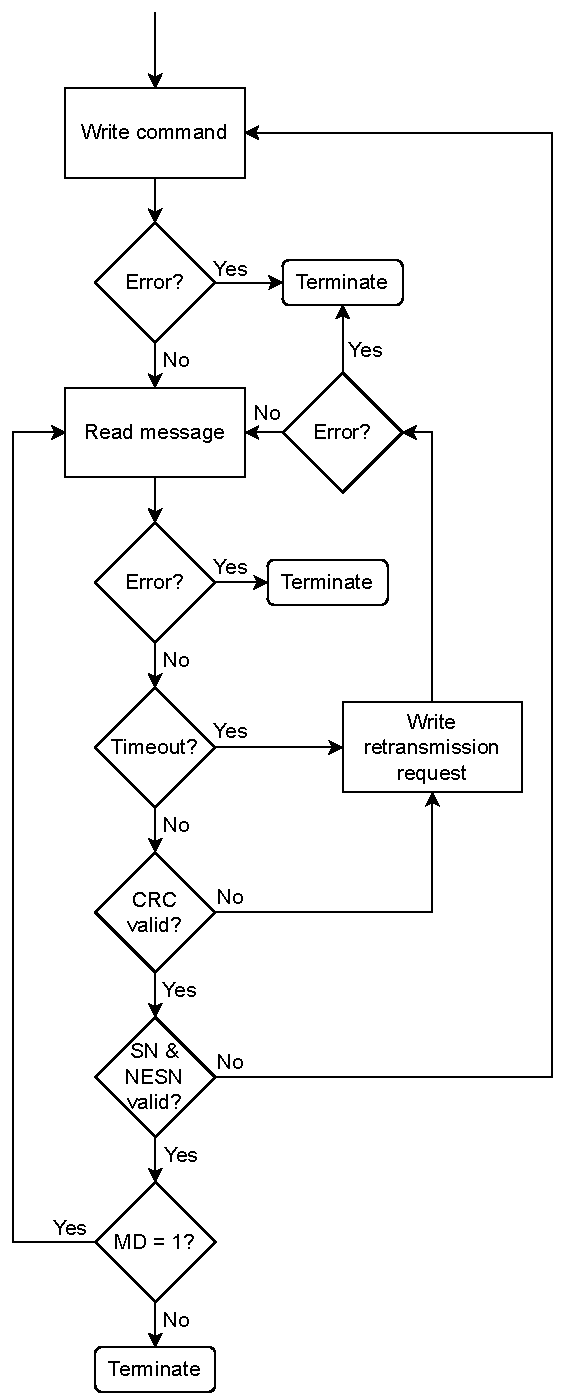
\includegraphics[width=0.4\textwidth]{figures/Bus_manager_diagram.pdf}
    \caption{High-level design diagram for serial writing using the bus manager}
    \label{fig:read_write_design}
\end{figure}

\begin{enumerate}
	\item \textbf{Write} the command to the serial bus.
	\item \textbf{Check for errors} after writing.
	\item \textbf{Read} the next incoming message.
	\item \textbf{Check for errors} after reading:
	\begin{itemize}
		\item Check for valid CRC
		\item Check for read timeout
	\end{itemize}
	\item \textbf{Send a retransmission request} and go to step 3 if an error occurred.
	\item \textbf{Check SN/NESN} message fields.
	\item \textbf{Retransmit the command} and go to step 3 if SN and/or NESN are invalid.
	\item \textbf{Send an ACK} packet to the serial bus.
	\item Go to step 3 if the MD field is set to 1.
\end{enumerate}

\subsection{Subsystem interfacing}
\label{sec:subsystem_interfacing}
The subsystem interfaces a bit differently, since it actively needs to listen for commands from the OBC or PPU. So it first reads from the bus, then uses the interfacing procedure described in Section \ref{sec:interfacing}.

%The overall design for interfacing between the host and controller is given in Figure \ref{fig:read_write_design}.
%We explain each step in a bit more detail below:
%\begin{itemize}
%	\item \textbf{Claim semaphore}: semaphore is claimed at the start of the sequence so response messages are not read by a different bus manager. We need to keep the semaphore until termination for the same reason: we don't want a bus manager to interrupt the message sequence. It is also crucial that the read/write operation is not interrupted, so we need to define a critical region \todo[inline]{How do we make sure the task is not preempted?}.
%	Lastly, we need to use a timeout for the semaphore claim. If a bus manager infinitely loops for some reason, we can never claim the semaphore and the whole system would lock up.
%	\item \textbf{Write message}: write a message to the serial bus and propagate any errors.
%	\item \textbf{Read message}: read a message from the serial bus. The read has a certain timeout specified by the programmer, which can be different for different messages. If the read times out an error is raised and the interfacing is terminated.
%	\item \textbf{Check CRC}: CRC is calculated over the payload in the response message and compared to the CRC inside the response message. If they do not match, the bus manager sends a retransmission request to the destination the response messasge came from. This is done until the bus manager runs out of retries or until the CRC is correct.
%	\item \textbf{Check ACK}: SN and NESN are checked to see if the request message was acknowledged or not. If it was not, the request message is retransmitted. This is done until the message is acknowledged or when the bus manager runs out of retries.
%	\item \textbf{Send ACK}: If everything in the message is correct, the bus manager sends an acknowledgement to the subsystem to indicate it received the message.
%	\item \textbf{Check MD}: if the MD bit is set, more data is on the way and we should read another message. This is done until MD is not set anymore.
%	\todo[inline]{Should we put a limit on the MD set? Because if it is always set you enter an infinite loop.}
%\end{itemize}

%\begin{figure}[h]
%	\centering
%	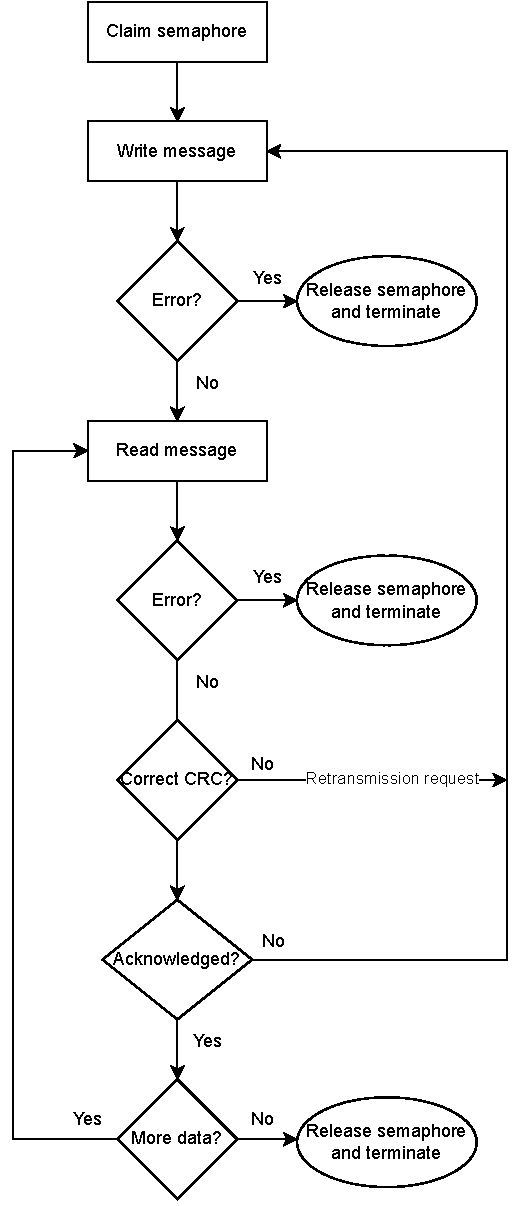
\includegraphics[width=0.3\textwidth]{figures/bus-manager-functional.drawio.pdf}
%    \caption{High-level design diagram for serial reading and writing using the bus manager}
%    \label{fig:read_write_design}
%\end{figure}


%\chapter{Implementation}

%\section{\texttt{Bus\_manager\_t} class}
%Each app will have its own \texttt{Bus\_manager\_t} instance to interface with its subsystem. The bus manager is used for reading and writing from and to one of the 5 serial buses that the OBC has access to. It is important to note that the \texttt{Bus\_manager\_t} class does NOT represent a bus, but merely a class that abstracts from reading and writing and that locks the bus from multiple accesses.
%\par Each of the buses have the following attributes. All of these are implemented as static arrays in the \texttt{Bus\_manager\_t} class.
%\begin{itemize}
	%\item \textbf{Named semaphore}: used to lock the bus to prevent multiple apps accessing the same bus at the same time.
	%\item \textbf{File descriptor}: used to read from and write to the bus. Must be locked using the semaphore before use.
	%\item \textbf{Initialisation variable}: used to indicate if the bus was initialised or not.
	%\item \textbf{State}: bus state. Not sure what this is used for yet.
%\end{itemize}

%\section{CRC calculation}
%We explain each step in a bit more detail below:
%\begin{itemize}
%	\item \textbf{Claim semaphore}: semaphore is claimed at the start of the %sequence so response messages are not read by a different bus manager. We need to keep the semaphore until termination for the same reason: we don't want a bus manager to interrupt the message sequence.
%	\item \textbf{Write message}: write a message to the serial bus and propagate any errors.
%	\item \textbf{Read message}: read a message from the serial bus. The read has a certain timeout specified by the programmer, which can be different for different messages. If the read times out an error is raised and the interfacing is terminated.
%	\item \textbf{Check CRC}: CRC is calculated over the payload in the response message and compared to the CRC inside the response message. If they do not match, the bus manager sends a retransmission request to the destination the response messasge came from.
%	\item \textbf{Check ACK}: SN and NESN are checked to see if the request message was acknowledged or not. If it was not, the request message is retransmitted. This is done until the message is acknowledged or when the bus manager runs out of retries.
%	\item \textbf{Check MD}: if the MD bit is set, more data is on the way and we should read another message. This is done until MD is not set anymore.
%	\todo[inline]{Should we put a limit on the MD set? Because if it is always set you enter an infinite loop.}
%\end{itemize}


\chapter{Implementation}
The implementation consists of two classes.
\begin{itemize}
	\item \texttt{Packet\_t} class: represents a message protocol packet.
	\item \texttt{Bus\_manager\_t} class: represents a bus manager for a single bus.
\end{itemize}
The bus manager class uses the packet class extensively to form packets for writing to the serial bus. Both classes are discussed below in more detail.

\section{\texttt{Packet\_t} class}
The packet class has the same instance variables as the fields of the messages that we use in the messaging protocol:
\begin{itemize}
	\item \texttt{preamble}: preamble field of the packet.
	\item \texttt{source}: source field of the packet.
	\item \texttt{destination}: source field of the packet.
	\item \texttt{pdu}: PDU field of the packet. Implemented as a struct with payload and header fields.
	\item \texttt{crc}: CRC field of the packet.
\end{itemize}
One of the reasons to have this class is that packets can be easily converted to and from raw bytes using a member function. The same is true for calculating the CRC of the packet.

\section{\texttt{Bus\_manager\_t} class}
\subsection{Members}
The bus manager has three public members:
\begin{itemize}
	\item \texttt{init}: implements the initialisation design from Section \ref{sec:initialisation}.
	\item \texttt{interface}: implements the interfacing design from Section \ref{sec:interfacing}.
	\item \texttt{read\_from\_bus}: used by subsystems to read from the bus before interfacing.
\end{itemize}
There are also some members that should be used to \textbf{interface to the specific serial bus code of the platform} (to be implemented by the programmer):
\begin{itemize}
	\item \texttt{configure\_serial}: should contain platform-specific code to configure the serial bus.
	\item \texttt{write\_to\_serial}: should contain platform-specific code to write to the serial bus.
	\item \texttt{read\_from\_serial}: should contain platform-specific code to read from the serial bus.
\end{itemize}

\subsection{Errors}
The bus manager class uses a \texttt{Result\_t} struct to indicate errors. It has an error code and error details. The errors should be forwarded to the app that sent the command. In Table \ref{tab:errors} we can see when which error occurs and what the details are.

\begin{table}[H]
\centering
\begin{tabular}{|p{6cm}|p{5.5cm}|p{3cm}|p{1cm}|}
	\hline
	\textbf{Situation} & \textbf{Error code} & \textbf{Error details} & \textbf{Fwd to app?} \\\hline
	Bus manager is already initialised & ALREADY\_INITIALISED & -- & Yes\\\hline
	Serial configuration failed & SERIAL\_CONFIGURE\_ERROR & configure error code & Yes\\\hline
	Serial write failed & SERIAL\_WRITE\_ERROR & write error code & Yes \\\hline
	Serial read failed & SERIAL\_READ\_ERROR & read error code & Yes \\\hline
	Serial read timeout & SERIAL\_TIMEOUT\_ERROR & -- & No \\\hline
	CRC invalid & INVALID\_CRC & crc & No \\\hline
	Too many retransmissions & RETRY\_LIMIT\_REACHED & NACK & Yes \\\hline
	Too many retransmission requests & RETRY\_LIMIT\_REACHED & previous error code & Yes \\\hline
	MD=1 but no more message expected & UNEXPECTED\_MULTIPLE\_DATA & --& Yes \\\hline
	NACK received & NACK & -- & No \\\hline
	Bus manager not initialised when interfacing & NOT\_YET\_INITIALISED & -- & Yes \\\hline
	Received packet destination not equal to subsystem & INVALID\_PACKET\_DESTINATION & previous error code & Yes \\\hline
	First received packet invalid (subsystem) & UNKNOWN\_PACKET\_DESTINATION & -- & Yes \\\hline
\end{tabular}
\caption{Situations where errors occur.}
\label{tab:errors}
\end{table}

%Each app will have its own \texttt{Bus\_manager\_t} instance to interface with its subsystem. The bus manager is used for reading and writing from and to one of the 5 serial buses that the OBC has access to. It is important to note that the \texttt{Bus\_manager\_t} class does NOT represent a bus, but merely a class that abstracts from reading and writing and that locks the bus from multiple accesses.
%\par Each of the buses have the following attributes. All of these are implemented as static arrays in the \texttt{Bus\_manager\_t} class.
%\begin{itemize}
%	\item \textbf{Named semaphore}: used to lock the bus to prevent multiple apps accessing the same bus at the same time.
%	\item \textbf{File descriptor}: used to read from and write to the bus. Must be locked using the semaphore before use.
%	\item \textbf{Initialisation variable}: used to indicate if the bus was initialised or not.
%	\item \textbf{State}: bus state. Not sure what this is used for yet.
%\end{itemize}
